\section{Bedingte Erwartungswerte und Martingale}

\subsection{Bedingte Dichte und bedingter Erwartungswert}

Motivation: Gegeben seien zwei Zufallsvariablen $(X,Y)$ mit Werten in $\R^m \times \Rn$ und gemeinsamer Dichte $f_{XY}(x,y)$.

Aus Dichte $f_{XY}$ können wir ableiten:
\begin{itemize}
	\item $f_Y(y) \defeq \int_{\R^m} f_{XY}(x,y) \dx$, die Randverteilung von $Y$
	\item $S_y \defeq \menge{y \in \Rn : f_Y(y) > 0}$, der Träger von $Y$
\end{itemize}

\begin{definition}
	Die bedingte Dichte von $X$ bzgl. $Y$ ist definiert als
	\begin{equation*}
	f_{X|Y}(x,y) = \begin{cases}
	\frac{f_{XY}(x,y)}{f_Y(y)} & y \in S_y \\ 0 & y \notin S_y
	\end{cases}
	\end{equation*}
\end{definition}

Betrachte folgende Problemstellung: Was ist die beste Vorhersage von $X$ gegeben eine Beobachtung $Y = y$?

Kriterium: Minimiere quadratischen Abstand bzw. das zweite Moment bzw. die $L_2$-Norm.

Vorhersage: messbare Funktion $\abb{g}{\Rn}{\R^m}, y \mapsto g(y)$.

\begin{equation}
\min\menge{\EW[(X-g(y))^2] : g \text{ messbar } \Rn \to \R^m} \tag{min-1} \label{eq: min-1}
\end{equation}

\begin{proposition} %1.3
	Wenn $(X,Y)$ eine gemeinsame Dichte besitzen und $\EW[\abs{X}^2] < \infty$ gilt, dann wird \eqref{eq: min-1} minimiert durch die bedingte Erwartung
	\begin{equation*}
	g(y) = \EW[X | Y=y] \defeq \int_{\R^m} x f_{X | Y}(x,y) \dx
	\end{equation*}
	Wir bezeichnen $ \EW[X | Y=y]$ als Erwartungswert von $X$ bedingt auf $Y=y$.
\end{proposition}

Allgemeiner gilt:

\begin{theorem} %1.4
	Seien $(X,Y)$ Zufallsvariablen mit gemeinsamer Dichte auf $\R^m \times \Rn$ und $\abb{h}{\R^m \times \Rn}{\R}$ messbar mit $\EW[h(X,Y)^2]$. Dann wird das Minimierungsproblem
	\begin{equation*}
	\min\menge{\EW[(h(X,Y)-g(Y))^2] : g \text{ messbar } \Rn \to \R}
	\end{equation*}
	gelöst durch
	\begin{equation*}
	g(y) = \EW[h(X,Y) | Y = y] = \int_{\R^m} h(x,y) * f_{X|Y}(x,y) \dx
	\end{equation*}
\end{theorem}

\begin{proof}[nur Proposition für $m=1$, Theorem analog]
	Setze $g(y) = \int_{\R} x f_{X|Y}(x,y) \dx$. Sei $\abb{p}{\Rn}{\R}$ eine beliebige messbare Funktion mit $\EW[p(Y)^2]< \infty$. Setze weiter $g_\epsilon(y) = g(y) + \epsilon p(y)$. Minimiere
	\begin{equation*}
	\begin{aligned}
		F(\epsilon) \defeq \EW[(X-g_\epsilon(Y))^2] 
		&= \EW[(X - g(Y) - \epsilon p(Y))^2] \\
		&= \EW[(X-g(Y))^2] - 2\epsilon \EW[(X-g(Y)) p(Y)] + \epsilon^2 \EW[p(Y)^2]
	\end{aligned}
	\end{equation*}
	Es ist
	\begin{equation*}
	\begin{aligned}
	\frac{\partial F}{\partial \epsilon}(\epsilon) &= 2\epsilon \EW[p(Y)^2] - 2\EW[(X-g(Y)) p(Y)]  \follows \epsilon_\ast \defeq\frac{\EW[(X-g(Y))p(Y)]}{\EW[p(Y)^2]} = \frac{A}{B} \\
	A &= \EW[Xp(Y)] - \EW[g(Y) p(Y)]  \\
	&= \int_{\R \times \Rn} x p(y) f_{XY}(x,y) \dx \dy - \int_{S_y} g(y) p(y) f_Y(y) \dy \\
	&= \int_{\R \times \Rn} x p(y) f_{XY}(x,y) \dx \dy - \int_{\R \times S_y} x p(y) \underbrace{f_{X|Y}(x,y) f_Y(y)}_{=f_{XY}(x,y)} \dy = 0
	\end{aligned}
	\end{equation*}
	Damit ist $\epsilon^\ast = 0$ unabhängig von $p$ und $g(y)$ minimiert \eqref{eq: min-1}.
\end{proof}

\begin{*beispiel}
	Seien $(X,Y)$ normalverteilt auf $\R \times \R$ mit
	\begin{equation*}
	\mu = \begin{pmatrix} \mu_X \\ \mu_Y \end{pmatrix} \qquad \Sigma 
	= \begin{pmatrix} \Var[X] & \Cov{X}{Y} \\ \Cov{X}{Y} & \Var[Y] \end{pmatrix}
	= \begin{pmatrix}
	\sigma_x^2 & \rho \sigma_x \sigma_y \\ \rho \sigma_x \sigma_y & \sigma_y^2
	\end{pmatrix}
	\qquad \rho \in [-1,1]
	\end{equation*}
	Dann ist die bedingte Dichte $f_{X|Y}(x,y)$ wieder die Dichte einer Normalverteilung mit
	\begin{equation*}
	\begin{aligned}
	\EW[X|Y=y] &= \mu_X + \rho \frac{\sigma_X}{\sigma_Y} \brackets{y - \mu_Y} \\
	\Var[X|Y=y] &= \sigma_X^2 (1-\rho^2)
	\end{aligned}
	\end{equation*}
	$\to$ siehe Übung.
	
	Die Abbildung $y \mapsto \mu_X + \rho \frac{\sigma_X}{\sigma_Y}(Y-\mu_Y)$ heißt Regressionsgerade für $X$ gegeben $Y = y$.
	Die Steigung wird im Wesentlichen durch $\rho$ bestimmt.
	
	\begin{center}
		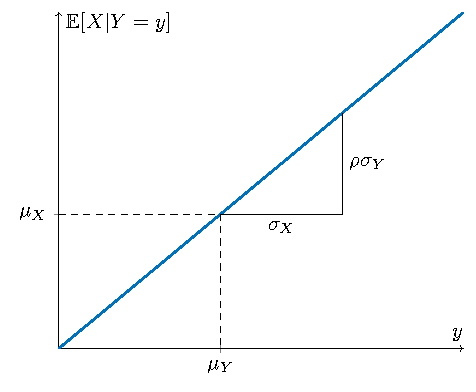
\includegraphics[width=.5\linewidth]{./img/bedingte-erwartung-regression}
		\captionof{figure}{Bedingte Erwartung als Regression}
	\end{center}
	
	Für diskrete Zufallsvariablen, d.h. wenn $X$,$Y$ nur endliche viele Werte $\menge{x_1, \dots , x_m}$ bzw. $\menge{y_1, \dots, y_n}$ annehmen, dann erhalten wir mit ähnlichen Überlegungen als Lösung von \eqref{eq: min-1} 
	\begin{equation*}
	\EW[X | Y=y_j] = \sum_{i=1}^m x_i \P(X=x_i | Y=y_j)
	\end{equation*}
	wobei direkt die bedingten Wahrscheinlichkeiten
	\begin{equation*}
	\P(X=x_i | Y=y_j) = \begin{cases}
	\frac{\P(X=x_i \land Y = y_j)}{\P(Y=y_j)} & \text{wenn } \P(Y = y_j) > 0 \\
	0 & \text{wenn } \P(Y=y_j) = 0
	\end{cases}
	\end{equation*}
	folgen.
\end{*beispiel}

\subsection{Bedingte Erwartung: Maßtheoretischer Zugang}

Wir betrachten den Wahrscheinlichkeitsraum $(\Omega, \F, \P)$. Für eine Zufallsvariable $\abb{X}{\Omega}{\R}$ und $p \in [1,\infty)$ definieren wir, die $L_p$-Norm
\begin{equation*}
\norm{X}_p \defeq \EW[\abs{X}^p]^{\frac{1}{p}} = \brackets{\int_\Omega \abs{X(\omega)}^p \diffskip{\P(\omega)}}^\frac{1}{p}
\end{equation*}
und den $L_p$-Raum
\begin{equation*}
L_p(\Omega, \F, \P) \defeq \menge{\abb{X}{\Omega}{\R} \enskip \F\text{-messbar}, \norm{X}_p < \infty}
\end{equation*}
Dabei identifizieren wir Zufallsvariablen, die sich nur auf $\P$-Nullmengen unterscheiden miteinander, d.h. $\P(X \neq X') = 0 \follows X = X'$ in $L_p$. Aus der Maßtheorie bekannt: Die Räume $L_p(\Omega,\F,\P)$ mit Norm $\norm{\dots}_p$ mit $p \in [1,\infty)$ sind
\begin{itemize}
	\item Banachräume, d.h. vollständige, normierte Vektorräume.
	\item für $p=2$ auch Hilbertraum mit innerem Produkt 
	\begin{equation*}
	\scal{X}{Y} = \EW[XY] = \int_\Omega X(\omega) Y(\omega) \diffskip{\P(\omega)}
	\end{equation*}
\end{itemize}

Für $\G \subseteq \F$ Unter-$\sigma$-Algebra ist $L_p(\Omega,\G,\P) \subseteq L_p(\Omega, \F, \P)$ ein abgeschlossener Unterraum.

Wir verallgemeinern das ''Vorhersageproblem`` aus dem letzten Abschnitt: Gegeben sei ein Zufallsvariale $X$ aus $L_2(\Omega,\F,\P)$ und $\G \subseteq \F$ eine Unter-$\sigma$-Algebra. Was ist die beste $\G$-messbare Vorhersage für $X$?

\begin{equation}
\min\menge{\EW[(X-G)^2] : G \in L_2(\Omega,\G,\P)} \tag{min-2} \label{eq: min-2}
\end{equation}

Aus der Hilbertraumtheorie folgt, dass \eqref{eq: min-2} eine eindeutige Lösung $G_\ast \in L_(\Omega, \G, \P)$ besitzt. $G_\ast$ ist die Orthogonalprojektion (bzgl. $\scal{\cdot}{\cdot}$) von $X \in L_2(\Omega,\F,\P)$ auf den abgeschlossenen Unterraum $L_2(\Omega,\G,\P)$.

% TODO Abbildung Hilbertraum

Wir bezeichnen $G_\ast \in L_2(\Omega, \F, \P)$ mit $\EW[X|\G]$ als bedingten Erwartunswert von $X$ bezüglich $\G$.

\begin{theorem} %1.5 
	\label{theorem: 1.5}
	Seien $X,Y \in L_2(\Omega,\F,\P)$ und $\G \subseteq \F$ eine Unter-$\sigma$-Algebra. Dann gilt
	\begin{itemize}
		\item Linearität: $\EW[aX + bY | \G] = a \EW[X|\G] + b\EW[Y|\G]$
		\item Turmregel: Für jede weitere $\sigma$-Algebra $\mathcal{H} \subseteq \G$ gilt ${\EW[{\EW[{X|\G}]}|\mathcal{H}]} = {\EW[X|\mathcal{H}]}$
		\item Pull-out-Property: $\EW[XZ|\G] = Z * \EW[X | \G]$ für alle beschränkten und $\G$-messbaren Zufallsvariablen $Z$.
		Für $Z$ $\G$-messbar mit $\EW[\abs{XZ}] < \infty$ gilt $\EW[XZ | \G] = Z * \EW[X | \G]$. Insbesondere gilt für $\G$-messbare $X$ schon $\EW[X|\G]=X$.
		\item Monotonie: $X \le Y \follows \EW[X|\G] \le \EW[Y|\G]$
		\item Dreiecksungleichung: $\abs{\EW[X|\G]} \le \EW[\abs{X}|\G]$
		\item Unabhängigkeit: $X$ unabhängig von $\G$ $\follows$ $\EW[X|\G] = \EW[X]$
		\item triviale $\sigma$-Algebra: $\G=\menge{\emptyset, \Omega} \follows \EW[X|\G] = \EW[X]$
	\end{itemize}
\end{theorem}
\begin{proof}
	siehe VL ''Wahrscheinlichkeitstheorie mit Martingalen``
\end{proof}

Die für $X \in L_2(\Omega,\F,\P)$ definierte bedingte Erwartung $\EW[X|\G]$ lässt sich durch Approximation auf alle $X \in L_1(\Omega,\F,\P)$ erweitern. Alle Eigenschaften aus \cref{theorem: 1.5} bleiben erhalten. 

Sei $Y$ eine Zufallsvariable und $\G= \sigma(Y)$ die von $Y$ erzeugte $\sigma$-Algebra. Wir schreiben $\EW[X|Y] = \EW[X|\sigma(Y)]$; dies ist eine $\G$-messbare Zufallsvariable.

Aus der Maßtheorie sag uns das Doob-Dynkin-Lemma, dass eine messbare Funktion $\abb{g}{\Rn}{\R}$ existiert, sodass $\EW[X|Y] = g(Y)$. Dabei ist $g$ genau die Funktion aus \eqref{eq: min-1}.

\paragraph{Zusammenfassung:}

Sei $X,Y$ aus $L_1(\Omega,\F,\P)$ und $\G \subseteq \F$ eine Unter-$\sigma$-Algebra. 
\begin{enumerate}[label=(\alph*),nolistsep,topsep=-\parskip]
	\item $\EW[X|Y=y]$ ist eine messbare Funktion $\abb{g}{\Rn}{\R^m}$ und falls eine bedingte Dichte existiert, dann gilt $\EW[X|Y=y] = \int_{\R^n} x f_{X|Y}(x,y) \dx$.
	\item $\EW[X|Y]$ ist eine $\sigma(Y)$-messbare Zufallsvariable und kann als $g(Y)$ dargestellt werden. Falls eine bedingte Dichte existiert, dann gilt $\EW[X|Y](\omega) = \int_\Rn x f_{X|Y}(x,Y(\omega)) \dx$.
	\item $\EW[X|\G]$ ist eine $\G$-messbare Zufallsvariable. Falls $\G=\sigma(Y)$ tritt Fall (b) ein.
\end{enumerate}
In allen Fällen kann $\EW[X|\cdot]$ interpretiert werden als \textit{beste Vorhersage} für $X$ gegeben
\begin{enumerate}[label=(\alph*),nolistsep,topsep=-\parskip]
	\item eine punktweise Betrachtung $Y=y$
	\item die Beobachtung $Y$
	\item die Information $\G$
\end{enumerate}

\subsection{Martingale}

Prototyp eines \enquote{neutralen} stochastischen Prozesses, der weder Aufwärts- noch Abwärtstrend besitzt. Wir betrachten hier den Prozess nur in diskreter Zeit $I = \N_0$.

\begin{definition}
	Sei $\folge{X}{n \in \N_0}$ ein stochastischer Prozess. Wenn gilt
	\begin{subequations}
		\begin{alignat}{2}
			\EW[\abs{X_n}] &< \infty \qquad &\forall n \in \N_0  \label{eq: martingal-a}\\
			\EW[X_{n+1}|X_1,\dots,X_n] &= X_n \qquad &\forall n \in \N_0 \label{eq: martingal-b}
		\end{alignat}
	\end{subequations}
	dann heißt $\folge{X_n}{n \in \N_0}$ \begriff{Martingal}.
\end{definition}

Wenn wir $\F_n^X = \sigma(X_1,\dots,X_n)$ definieren, können wir \eqref{eq: martingal-b} schreiben als 
\begin{equation*}
	\EW[X_{n+1}|\F_n^X] = X_n \qquad \forall n \in \N
\end{equation*}

\textbf{Konvention}: Alle stochastischen Prozesse $\folge{X_n}{n \in \N_0}$ haben deterministischen Startwert $X_0$.

Interpretation: Die beste Vorhersage für den zukünftigen Wert $X_{n+1}$ basierend auf der Vergangenheit $\sigma(X_1,\dots,X_n)$ ist der momentane Wert $X_n$.
Aus der Turmregel folgt:
\begin{equation*}
	\EW[X_{n+k}|\F_n^X] = X_n \qquad \forall n,k \in \N_0 %b''
\end{equation*}
denn
\begin{equation*}
	\EW[X_{n+k}|\F_n^X] = \EW[\underbrace{\EW[X_{n+k}|\F_{n+k-1}^X]}_{=X_{n+k-1}}|\F_n^X] = \EW[X_{n+k-1}|\F_n^X] \overset{k \text{ mal}}{=} X_n
\end{equation*}

Man kann von $\folge{\F_n^X}{n \in \N}$ auf beliebige Filtrationen $\folge{\F_n}{n \in \N_0}$ erweitern.

\begin{*definition}
	Sei $\folge{X_n}{n \in \N_0}$ ein stochastischer Prozess, adaptiert an eine Filtration $\folge{\F_n}{n \in \N_0}$. Wenn gilt
	\begin{alignat}{2}
		\EW[\abs{X_n}] &< \infty \qquad &\forall n \in \N_0 \tag{a} \label{eq: martingal-ad-a}\\
		\EW[X_{n+1}|\F_n] &= X_n \qquad &\forall n \in \N_0  \tag{b} \label{eq: martingal-ad-b}
	\end{alignat}
	dann heißt $\folge{X_n}{n \in \N_0}$ Martingal bezüglich der Filtration $\folge{\F_n}{n \in \N_0}$.
\end{*definition}

Interpretation: Beste Vorhersage für zukünftigen Wert $X_{n+1}$, basierend auf verfügbarer Information $\F_n$ ist der momentane Wert $X_n$.

\begin{*definition}
	Falls in Punkt \eqref{eq: martingal-ad-b} statt ''$=$`` die Ungleichung ''$\le$`` oder ''$\ge$`` gilt, so heißt $\folge{X_n}{n \in \N}$ \begriff{Super- bzw. Submartingal}.
\end{*definition}

\begin{itemize}
	\item Wenn $X=\folge{X_n}{n \in \N}$ ein Martingal ist, dann gilt $\EW[X_n] = X_0$, d.h. $n \mapsto \EW[X_n]$ ist konstant. Begründung:
	\begin{equation*}
		\EW[X_{n+1}|\F_n] = X_n \follows \underbrace{\EW[{\EW[X_{n+1}|\F_n]}]}_{= \EW[X_{n+1}]} = \EW[X_n] \overset{n \text{ mal}}{\follows} \EW[X_n] = X_0
	\end{equation*}
	\item $X$ Submartingal $\follows n \mapsto \EW[X_n]$ ist monoton steigend
	\item $X$ Supermartingal $\follows n \mapsto \EW[X_n]$ ist monoton fallend
\end{itemize}

\enquote{Das Leben ist ein Supermartingal -- die Erwartungen fallen mit der Zeit} \smiley

\begin{beispiel}
	Seien $\folge{Y_n}{n \in \N}$ unabhängige Zufallsvariablen in $L_1(\Omega,\F,\P)$ mit $\EW[Y_n] = 0$. Betrachten wir die Partialsummen $X_n \defeq \sum_{k=1}^n Y_k$ und $X_0 = 0$. Dann ist $\folge{X_n}{n \in \N_0}$ ein Martingal, denn
		\begin{equation*}
			\begin{aligned}
			\EW[\abs{X_n}] &\le \sum_{k=1}^n \EW[\abs{Y_k}] < \infty \qquad \forall n \in \N \\
			\EW[X_{n+1} \mid \F_n^X] &= \EW[Y_{n+1} + X_n \mid \F_n^X] \\
			&= \EW[Y_{n+1} \mid \F_n^X] + \EW[X_n \mid \F_n^X] = \underbrace{\EW[Y_{n+1}]}_{=0} + X_n \\
			&= X_n
			\end{aligned}
		\end{equation*}
\end{beispiel}

\begin{*definition}
	Sei $\folge{\F_n}{n \in \N_0}$ eine Filtration. Ein stochastischer Prozess $\folge{H_n}{n \in \N}$ heißt \begriff{vorhersehbar} [predictable] bezüglich $\folge{\F_n}{n \in \N_0}$ wenn gilt
	\begin{equation*}
		H_n \text{ ist } \F_{n-1} \text{-messbar} \qquad \forall n \in \N
	\end{equation*}
\end{*definition}

\begin{*bemerkung}
	Vorhersehbarkeit ist eine stärkere Eigenschaft als Adaptiertheit.
\end{*bemerkung}

\begin{*definition}
	Sei $X$ ein adaptierter und $H$ ein vorhersehbarer stochastischer Prozess bezüglich $\folge{\F_n}{n \in \N}$. Dann heißt 
	\begin{equation}
		(H \bullet X)_n \defeq \sum_{k=1}^n H_k (X_k - X_{k-1}) \tag{$\star$} \label{eq: diskretesIntegral}
	\end{equation}
	\begriff{diskretes stochastisches Integral} von $H$ bezüglich $X$.
\end{*definition}

\begin{*bemerkung}
	Summen \eqref{eq: diskretesIntegral} heißen in der Analysis Riemann-Stieltjes-Summen und werden für die Konstruktion des Riemann-Stieltjes-Integrals $\int h \diffskip{\rho}$ verwendet.
\end{*bemerkung}

\begin{*definition}
	Ein stochastischer Prozess $\folge{H_n}{n \in \N}$ heißt \begriff{lokal beschränkt}, wenn eine deterministische Folge $c_n \in \R_{\ge 0}$ existiert, sodass
	\begin{equation*}
		\abs{H_n} \le c_n \enskip \text{ fast sicher } \qquad \forall n \in \N
	\end{equation*}
\end{*definition}

\begin{satz} %1.6
	Sei $X$ adaptierter stochastischer Prozess (bezüglich Filtration $\folge{\F_n}{n \in \N}$). Dann sind äquivalent:
	\begin{enumerate}
		\item $X$ ist Martingal bezüglich $\folge{\F_n}{n \in \N}$.
		\item $(H \bullet X)$ ist Martingal für alle lokal beschränkten, vorhersbaren Prozesse $H$
	\end{enumerate}
\end{satz}

Das stochastische Integral erhält also die Martingaleigenschaft.

\begin{proof}
    \begin{equivalence}
        \hinrichtung $(H \bullet X)_n = \sum_{k=1}^n H_k (X_k - X_{k-1})$.
        \begin{itemize}
            \item Adaptiertheit: klar
            \item Integrierbarkeit: $H$ lokal beschränkt, d.h. $\abs{H_k} \le c_k < \infty$ für alle $k$.
            \begin{equation*}
                \EW[\abs{H_k (X_k - X_{k-1})}] \le c_k * \brackets{\EW[\abs{X_k}] + \EW[\abs{X_{k-1}}]} < \infty
            \end{equation*}
            Mit der Dreiecksungleichung folgt daraus $\EW[\abs{(H \bullet X)_n}] < \infty$.
            \item Martingaleigenschaft: 
            \begin{equation*}
                \begin{aligned}
                    \EW[(H \bullet X)_n \mid \F_{n-1}] &
                    = (H \bullet X)_{n-1} + \EW[H_n (X_n - X_{n-1}) \mid \F_{n-1}] \\
                    & = (H \bullet X)_{n-1} + H_n * \underbrace{\brackets{\EW[X_n \mid \F_{n-1}] - X{n-1}}}_{=0} \\
                    & = (H \bullet X)_{n-1} \quad \forall n \in \N
                \end{aligned}
            \end{equation*}
            Damit ist also auch $(H \bullet X)$ ein Martingal.		
        \end{itemize}
        \rueckrichtung Fixiere $N \in \N$. Setze $H_n \defeq \one_{n = N}$, dieser ist lokal beschränkt und deterministisch (also auch vorhersehbar). Man stellt fest, dass $(H \bullet X)_n = 0$ für alle $n \le N-1$. Für alle $n \ge N$ gilt dagegen $(H \bullet X)_n = X_N - X_{N-1}$. Wir überprüfen nur die Martingaleigenschaft (Integrierbarkeit folgt aus Dreiecksungleichung). Wir wissen, dass $(H \bullet X)$ ein Martingal ist. 
        \begin{align*}
            0 = (H \bullet X)_{N-1} 
            = \EW[(H \bullet X)_N \mid \F_{N-1}]
            & = \EW[X_N - X_{N-1} \mid \F_{N-1}] \\
            & = \EW[X_N \mid \F_{N-1}] - X_{N-1} \\
            \follows X_{N-1} &= \EW[X_N \mid \F_{N-1}] \mit N \in \N \text{ beliebig}
        \end{align*}
        Somit ist $X$ ein Martingal.
    \end{equivalence}
\end{proof}

\begin{korollar} %1.7
	Sei $X = \folge{X_n}{n=1 , \dots, N}$ ein adaptierter stochastischer Prozess bezüglich einer Filtration $\folge{\F_n}{n=1 , \dots, N}$. Wenn $\EW[(H \bullet X)_N] = 0$ für alle lokal beschränkten vorhersehbaren Prozesse $H$, dann ist $X$ ein Martingal bezüglich $\folge{\F_n}{}$.
\end{korollar}
\begin{proof}
	Fixiere $K \in  [N] \defeq \menge{1, 2, \dots , N}$ und eine Menge $A \in \F_{K-1}$. Definiere $H_n(\omega) = \one_A (\omega) * \one_{\menge{n=K}}$, dieser ist lokal beschränkt und vorhersehbar.
	Es ist $(H \bullet X)_n = 0$ für alle $n \le K-1$. Für alle $n \ge K$ gilt $(H \bullet X)_n = \one_A * (X_K - X_{K-1})$. 
	\begin{align*}
		0 = \EW[(H \bullet X)_N] 
		&= \EW[\one_A (X_K - X_{K-1})] \\
		\overset{\text{Turm}}&{=} \EW[{\EW[\one_A (X_K - X_{K-1}) \mid \F_{K-1}]}] \\
		&= \EW[ \one_A *  \underbrace{ \brackets{\EW[X_K \mid \F_{K-1}] - X_{K-1}}}_{\defqe Y_{K-1}} ] \quad \forall A \in \F_{K-1} \\
		\follows \int_A  Y_{K-1}(\omega) \diff{\P(\omega)} &= \int_A X_{K-1}(\omega) \diff{\P(\omega)} \quad \forall A \in \F_{K-1} \\
		\follows Y_{K-1} &= X_{K-1} \text{ fast sicher} \\
		\follows \EW[X_K \mid \F_{K-1}] - X_{K-1} &= X_{K-1}
	\end{align*}
	für beliebige $K$. Somit ist $X$ ein Martingal.
\end{proof}

\begin{bemerkung}
	Wir schreiben $[N] \defeq \menge{1, 2, \dots, N}$ und $[N]_0 \defeq \menge{0, 1, 2 , \dots , N}$.
\end{bemerkung}
